\documentclass[10pt,xcolor=svgnames]{beamer}
\usepackage{palatino} %font type
\usepackage{appendixnumberbeamer}
\usefonttheme{metropolis} %Type of slides
\usefonttheme[onlymath]{serif} %font type Mathematical expressions
\usetheme[progressbar=frametitle,titleformat frame=smallcaps,numbering=counter]{metropolis} %This adds a bar at the beginning of each section.
\useoutertheme[subsection=false]{miniframes} %Circles in the top of each frame, showing the slide of each section you are at

 %enumerate each slide without counting the appendix
\setbeamercolor{progress bar}{fg=Maroon!70!Coral} %These are the colours of the progress bar. Notice that the names used are the svgnames
\setbeamercolor{title separator}{fg=DarkSalmon} %This is the line colour in the title slide
\setbeamercolor{structure}{fg=black} %Colour of the text of structure, numbers, items, blah. Not the big text.
\setbeamercolor{normal text}{fg=black!87} %Colour of normal text
\setbeamercolor{alerted text}{fg=DarkRed!60!Gainsboro} %Color of the alert box
\setbeamercolor{example text}{fg=Maroon!70!Coral} %Colour of the Example block text


\setbeamercolor{palette primary}{bg=NavyBlue!50!DarkOliveGreen, fg=white} %These are the colours of the background. Being this the main combination and so one. 
\setbeamercolor{palette secondary}{bg=NavyBlue!50!DarkOliveGreen, fg=white}
\setbeamercolor{palette tertiary}{bg=NavyBlue!40!Black, fg= white}
\setbeamercolor{section in toc}{fg=NavyBlue!40!Black} %Color of the text in the table of contents (toc)

\usepackage{amsmath,amssymb}
\usepackage{slashed}
\usepackage{cite}
\usepackage{relsize}
\usepackage{caption}
\usepackage{subcaption}
\usepackage{multicol}
\usepackage{booktabs}
\usepackage[scale=2]{ccicons}
\usepackage{pgfplots}
\usepgfplotslibrary{dateplot}
\usepackage{geometry}
\usepackage{xspace}
\usepackage[brazilian]{babel}
\usepackage[letterspace=200]{microtype}
\newcommand{\themename}{\textbf{\textsc{bluetemp}\xspace}}%metropolis}}\xspace}

\title{Classificação morfológica de galáxias usando conjunto de redes neurais convolucionais}
\author[Name]{Natanael Magalhães Cardoso$^{*}$\\ Profa. Cláudia Mendes de Oliveira$^{\dagger}$}
% \subtitle{Subtitle}
\institute[uni]{$^{*}$ Departamento de Computação e Sistemas Digitais, Escola Politécnica, USP\\$^{\dagger}$ Departamento de Astronomia, Instituto de Astronomia, Geofísica e Ciências Atmosféricas, USP}
\date{}
% \titlegraphic{\vspace{-0.5cm}\hfill
\includegraphics[height=37mm]{figures/urania_color.pdf}} %You can modify the location of the logo by changing the command \vspace{}. 

\begin{document}
{
\setbeamercolor{background canvas}{bg=NavyBlue!50!DarkOliveGreen, fg=white}
\setbeamercolor{normal text}{fg=white}
\maketitle
}

\metroset{titleformat frame=smallcaps} %This changes the titles for small caps

{
  \AtBeginSection{}
  \section{Introdução}
}

\begin{frame}{Background: Astronomia}
  \begin{minipage}{0.4\textwidth}
    \begin{figure}
      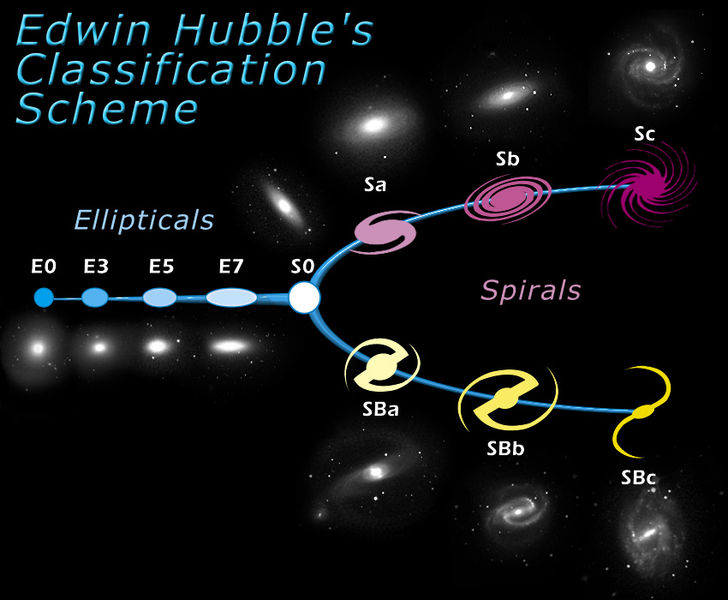
\includegraphics[width=\linewidth]{fig/tunning-fork.jpg}
      \caption{Hubble's Tunning Fork}
    \end{figure}
  \end{minipage}\hfill
  \begin{minipage}{0.54\textwidth}
    \begin{figure}
      \begin{tabular}{cc}
        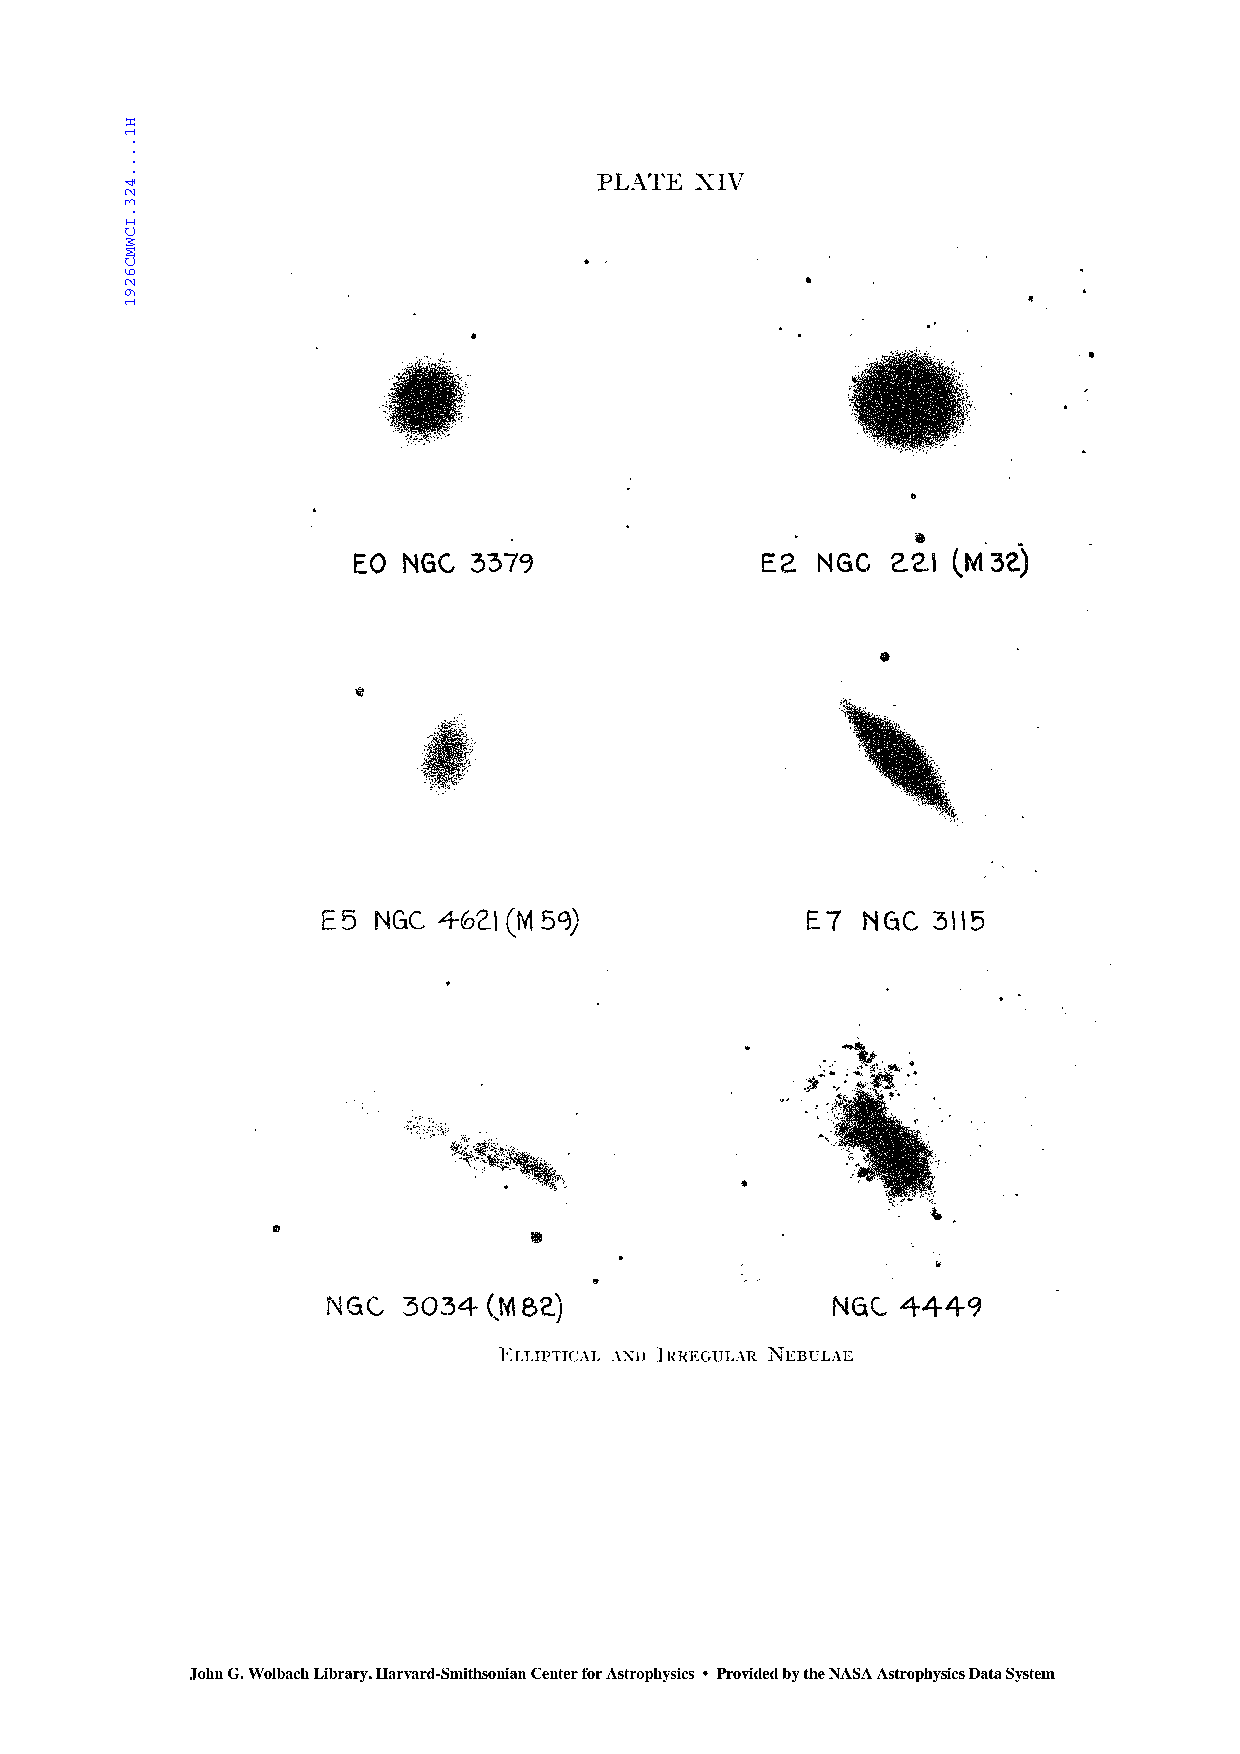
\includegraphics[width=0.49\linewidth,trim={50mm 65mm 35mm 55mm},clip]{papers/hubble-5.pdf} & 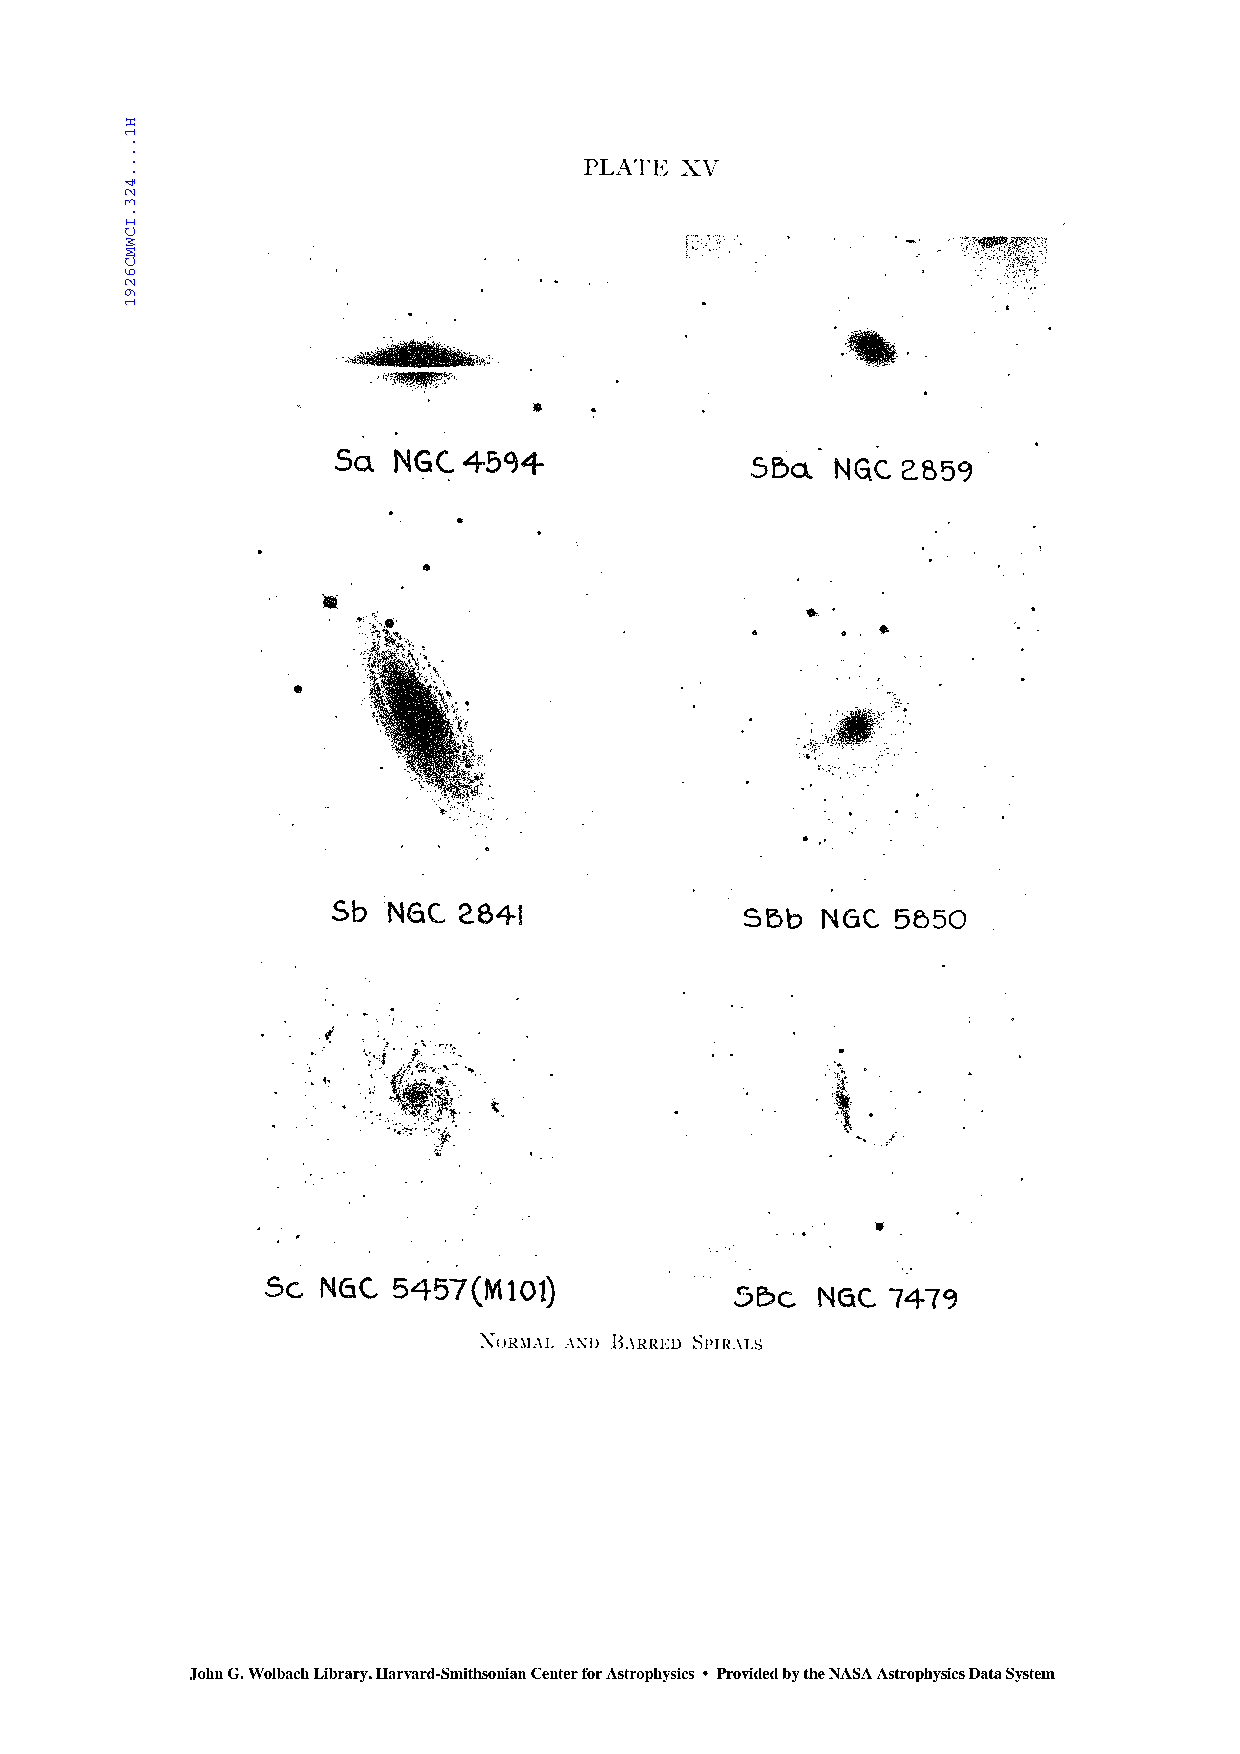
\includegraphics[width=0.49\linewidth,trim={50mm 65mm 35mm 55mm},clip]{papers/hubble-8.pdf}
      \end{tabular}
      \caption{Extragalactic Nebulae; E. Hubble, 1926.}
    \end{figure}
  \end{minipage}
\end{frame}

\begin{frame}{Background: Neurociência}
  \begin{figure}
    \begin{tabular}{cc}
      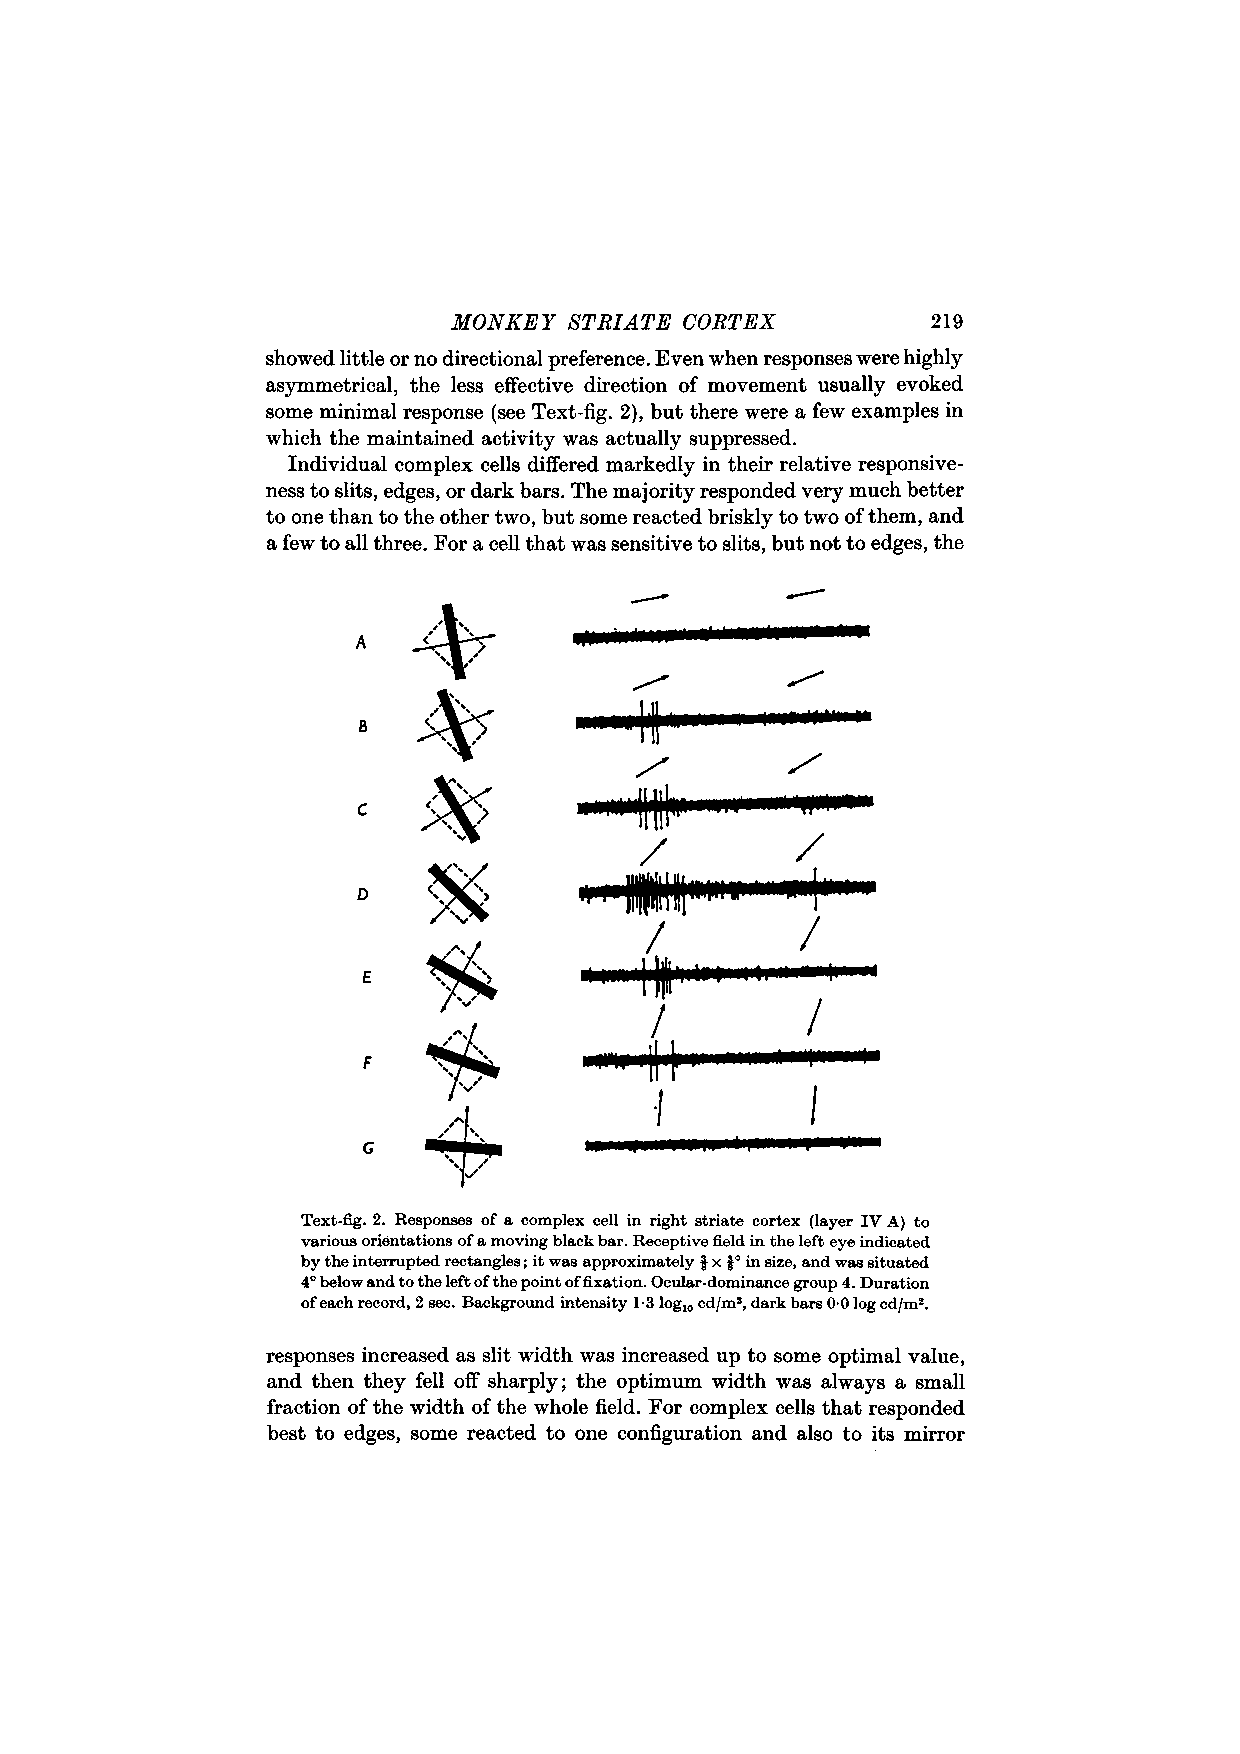
\includegraphics[width=0.38\linewidth,trim={42mm 65mm 45mm 50mm},clip]{papers/hubel-5.pdf} & 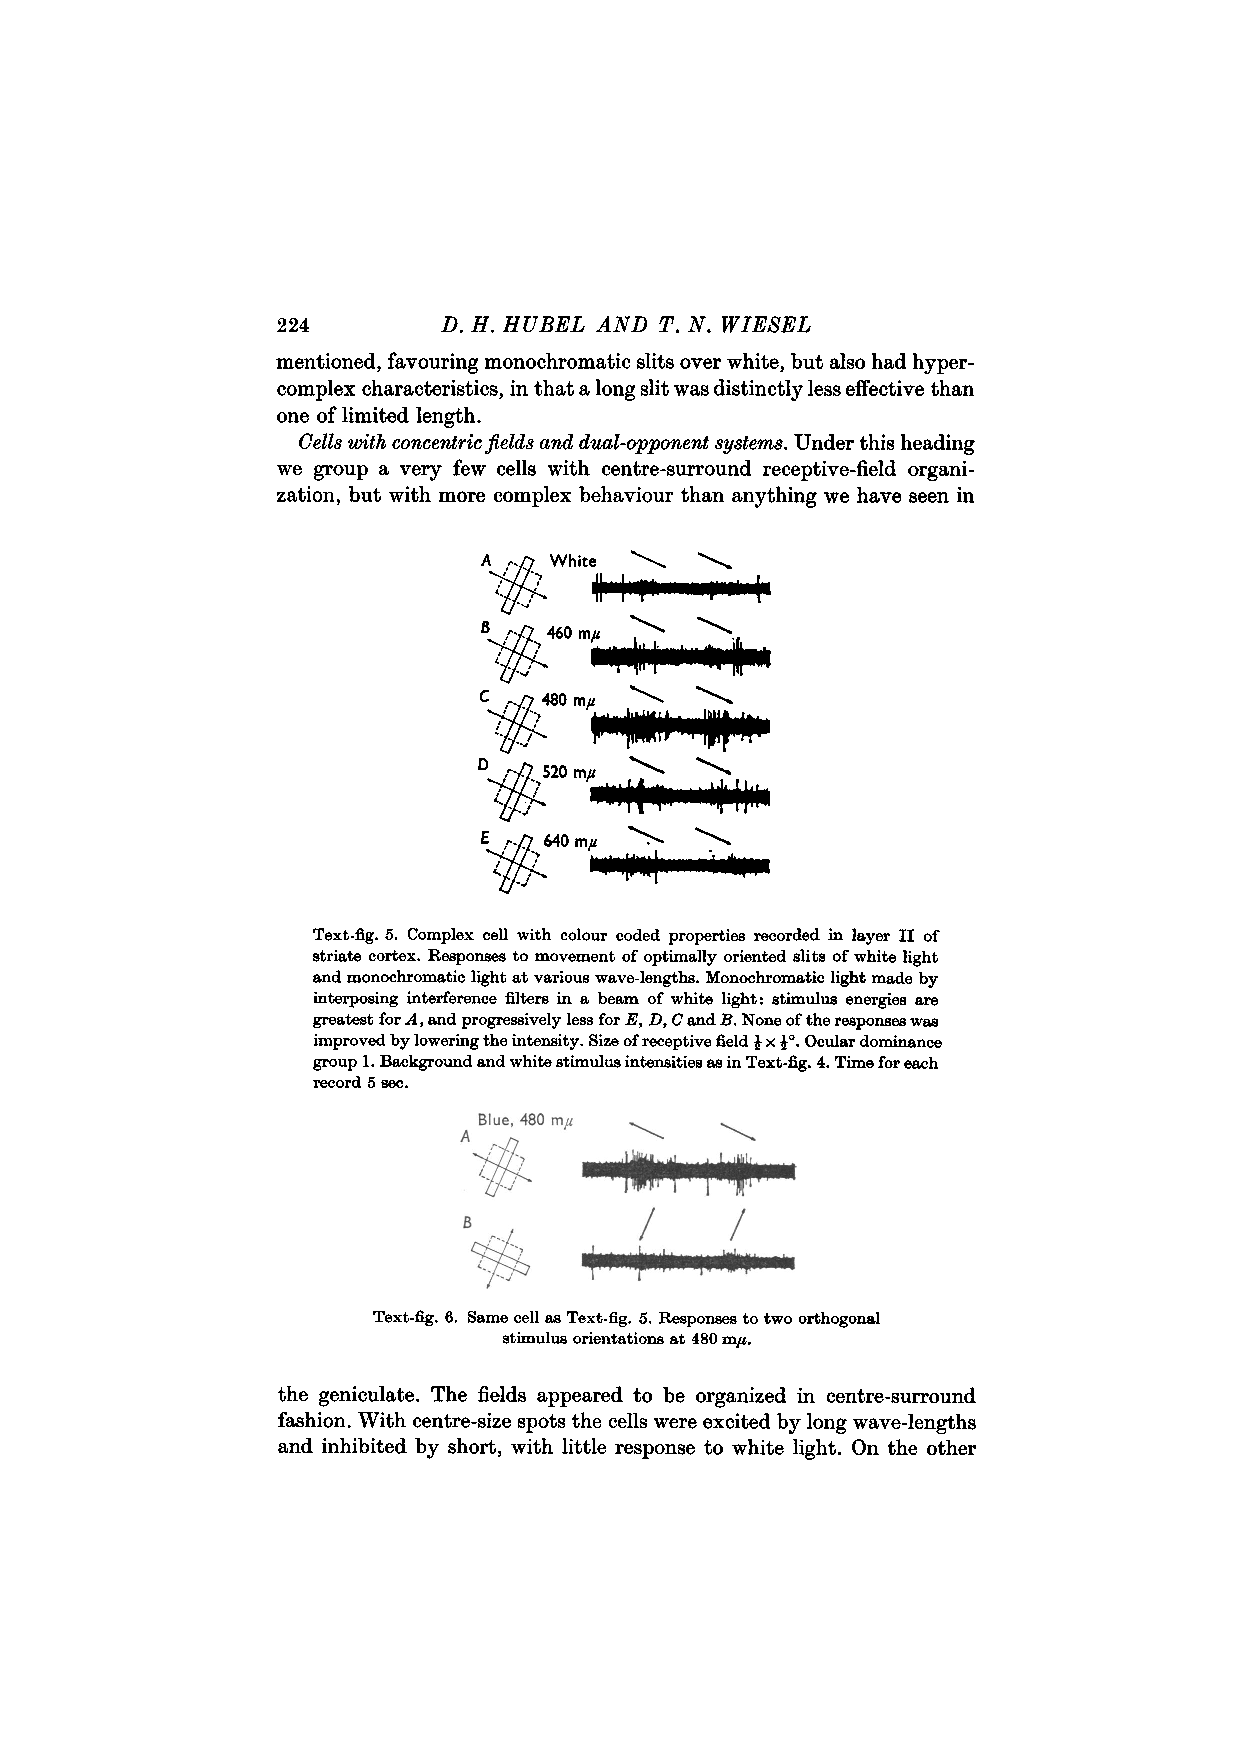
\includegraphics[width=0.38\linewidth,trim={42mm 65mm 45mm 50mm},clip]{papers/hubel-10.pdf}
    \end{tabular}
    \caption{Monkey Striate Cortex; D. H. Hubel \& T. N. Wisel, 1968.}
  \end{figure}
\end{frame}

\begin{frame}{Background: Visão Computacional}
  \begin{figure}
    \begin{tabular}{cc}
      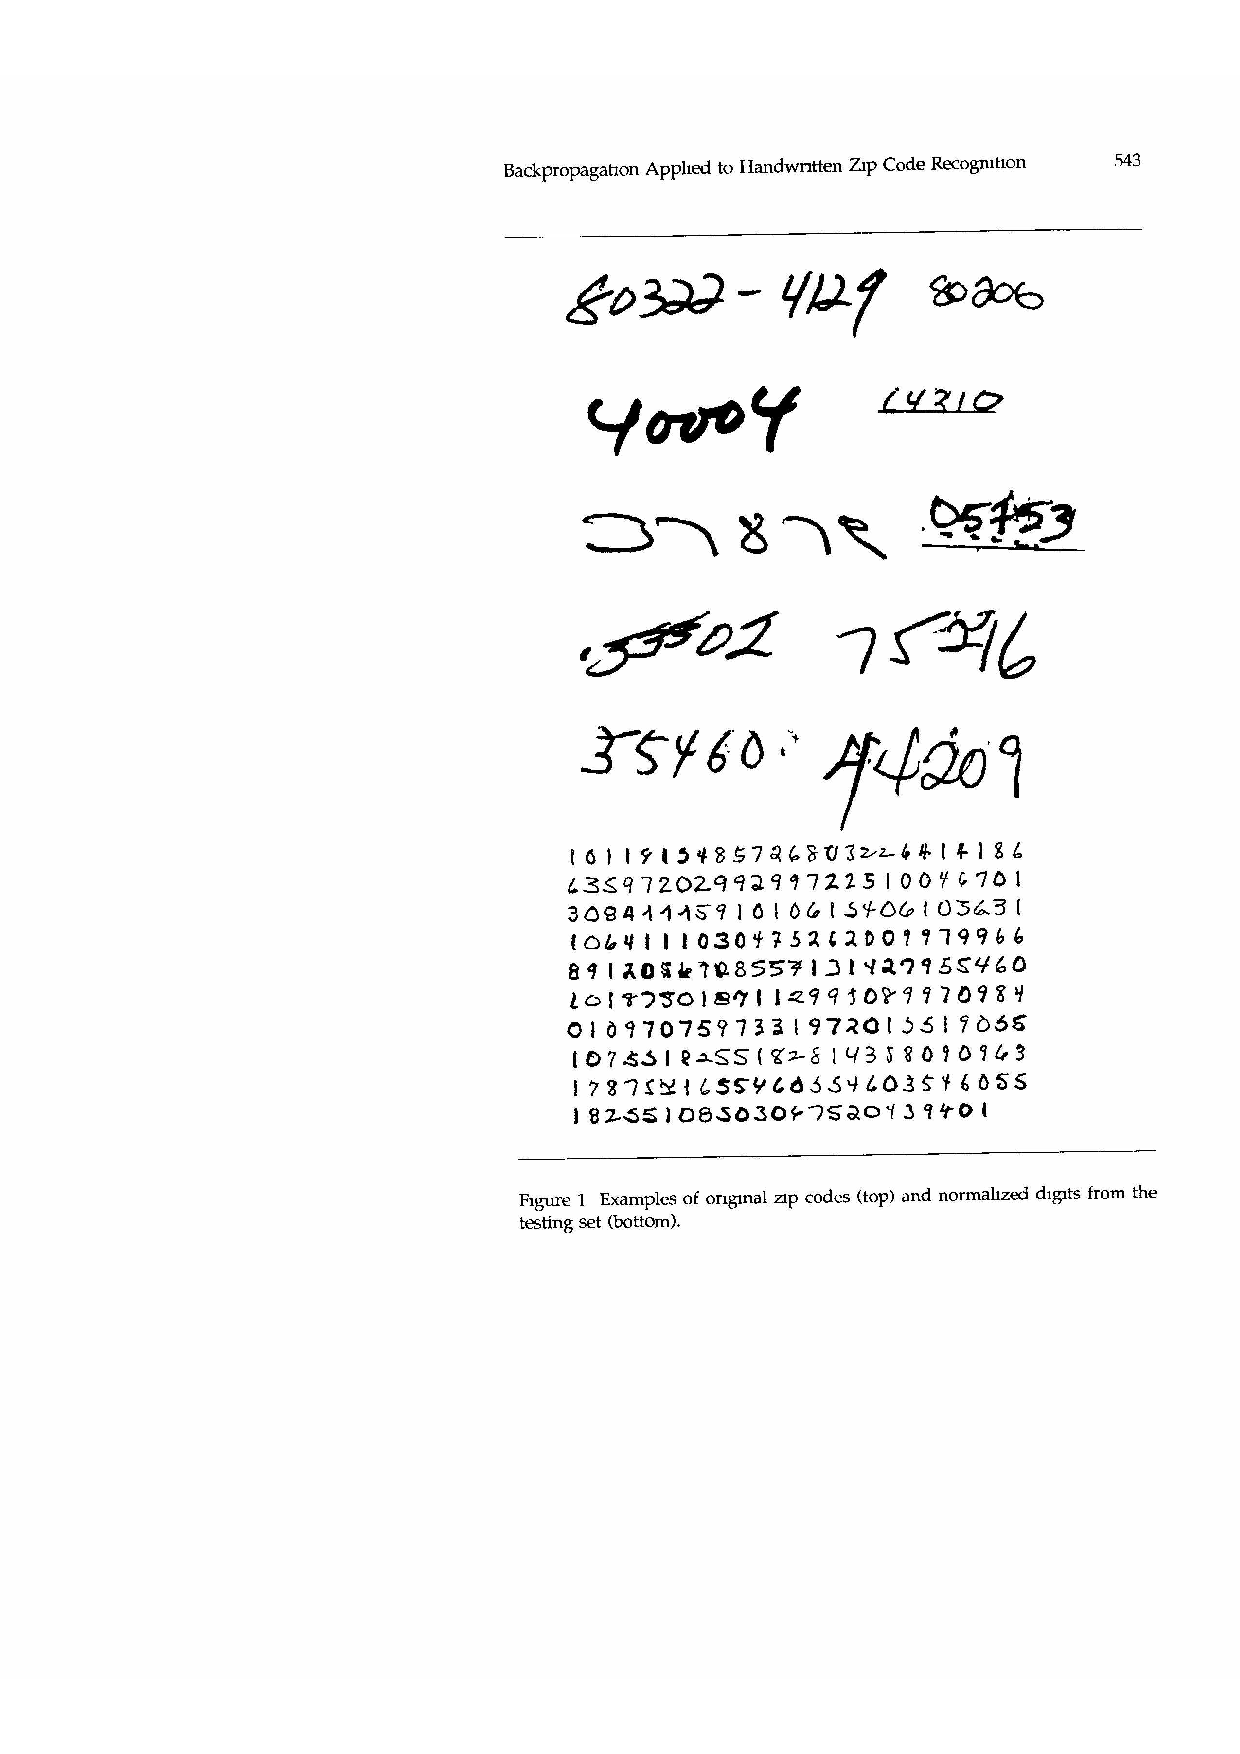
\includegraphics[height=0.76\textheight,trim={85mm 85mm 20mm 20mm},clip]{papers/lecun-3.pdf} & 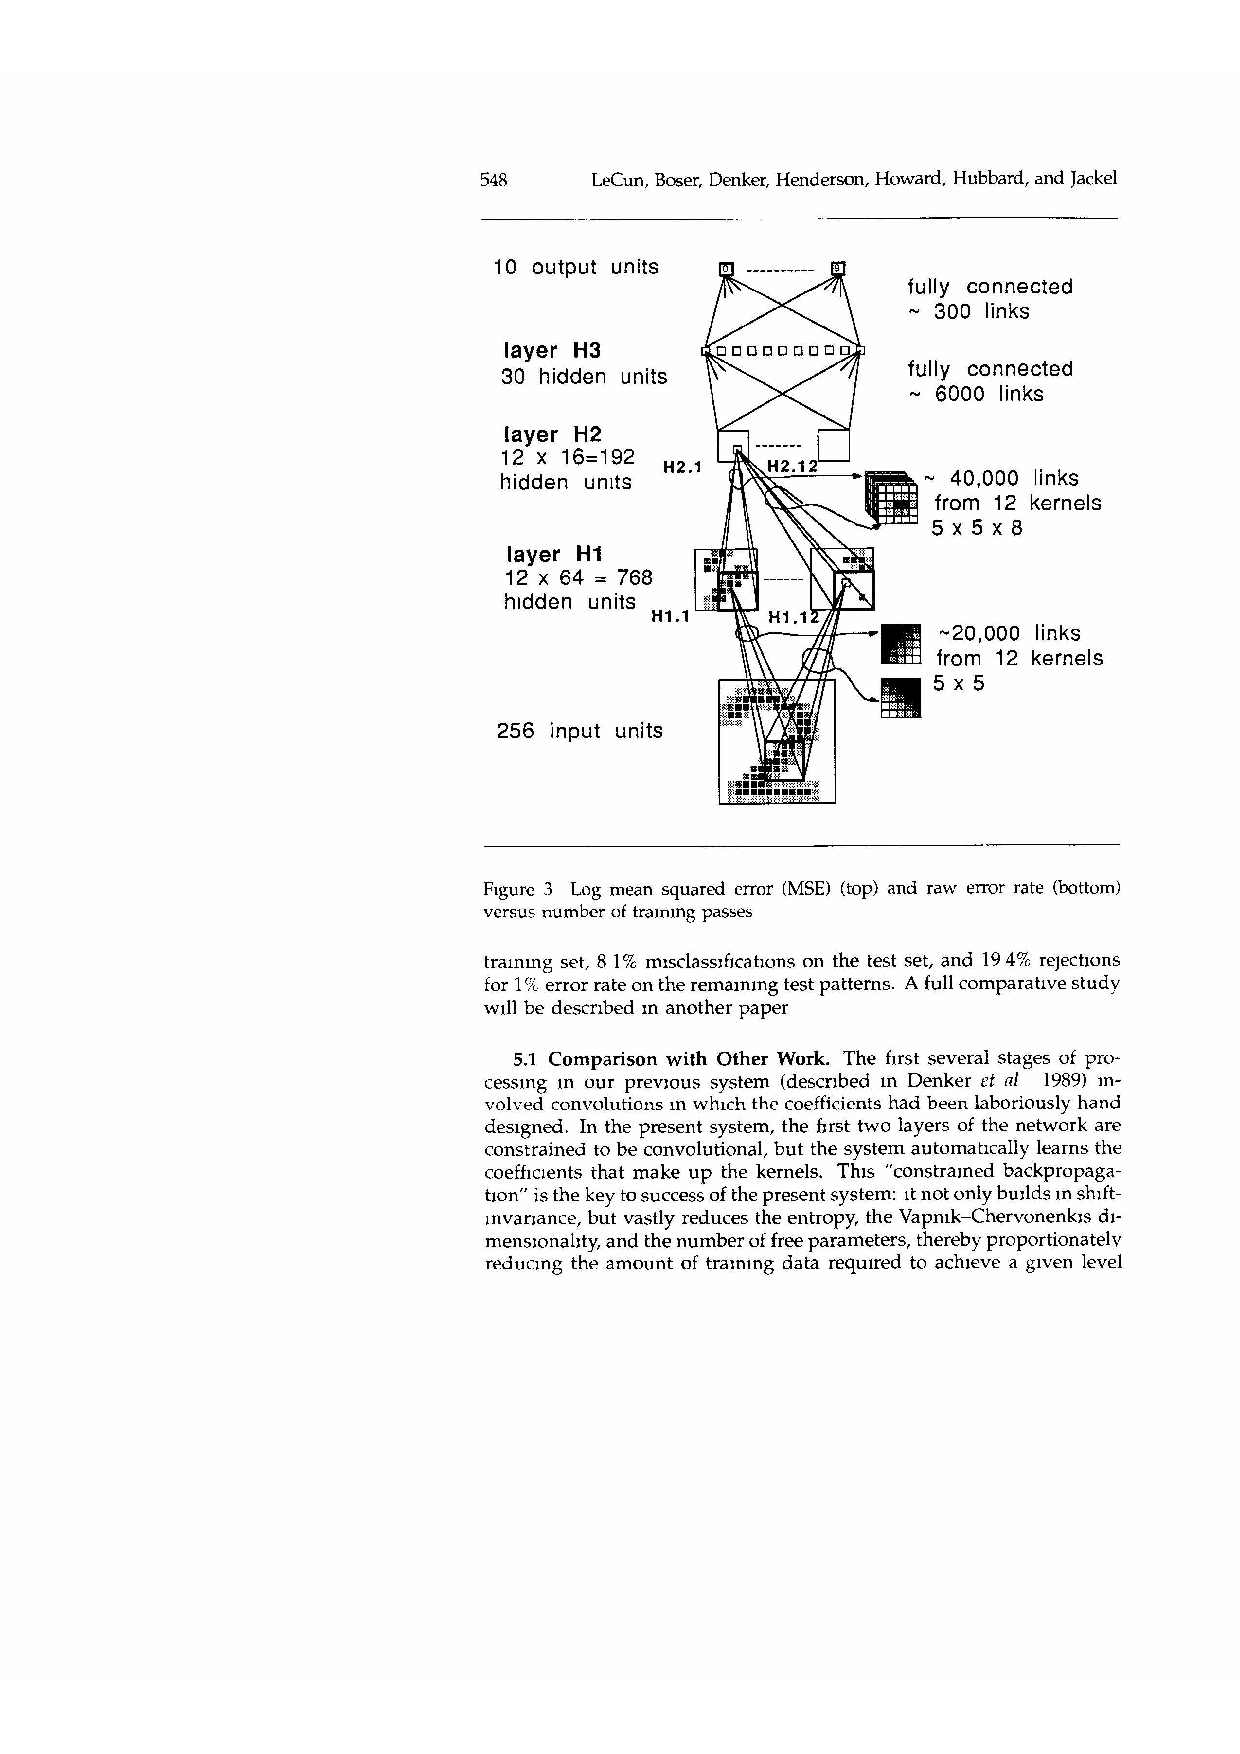
\includegraphics[height=0.76\textheight,trim={80mm 80mm 18mm 20mm},clip]{papers/lecun-8.pdf}
    \end{tabular}
    \caption{Backpropagation applied to Handwritten Zip Code Recognition; Y. LeCun et al., 1989.}
  \end{figure}
\end{frame}

\begin{frame}{Objetivo}
  \begin{minipage}{0.48\textwidth}
    \begin{center}
      \textbf{Problema}
    \end{center}
    \begin{figure}
      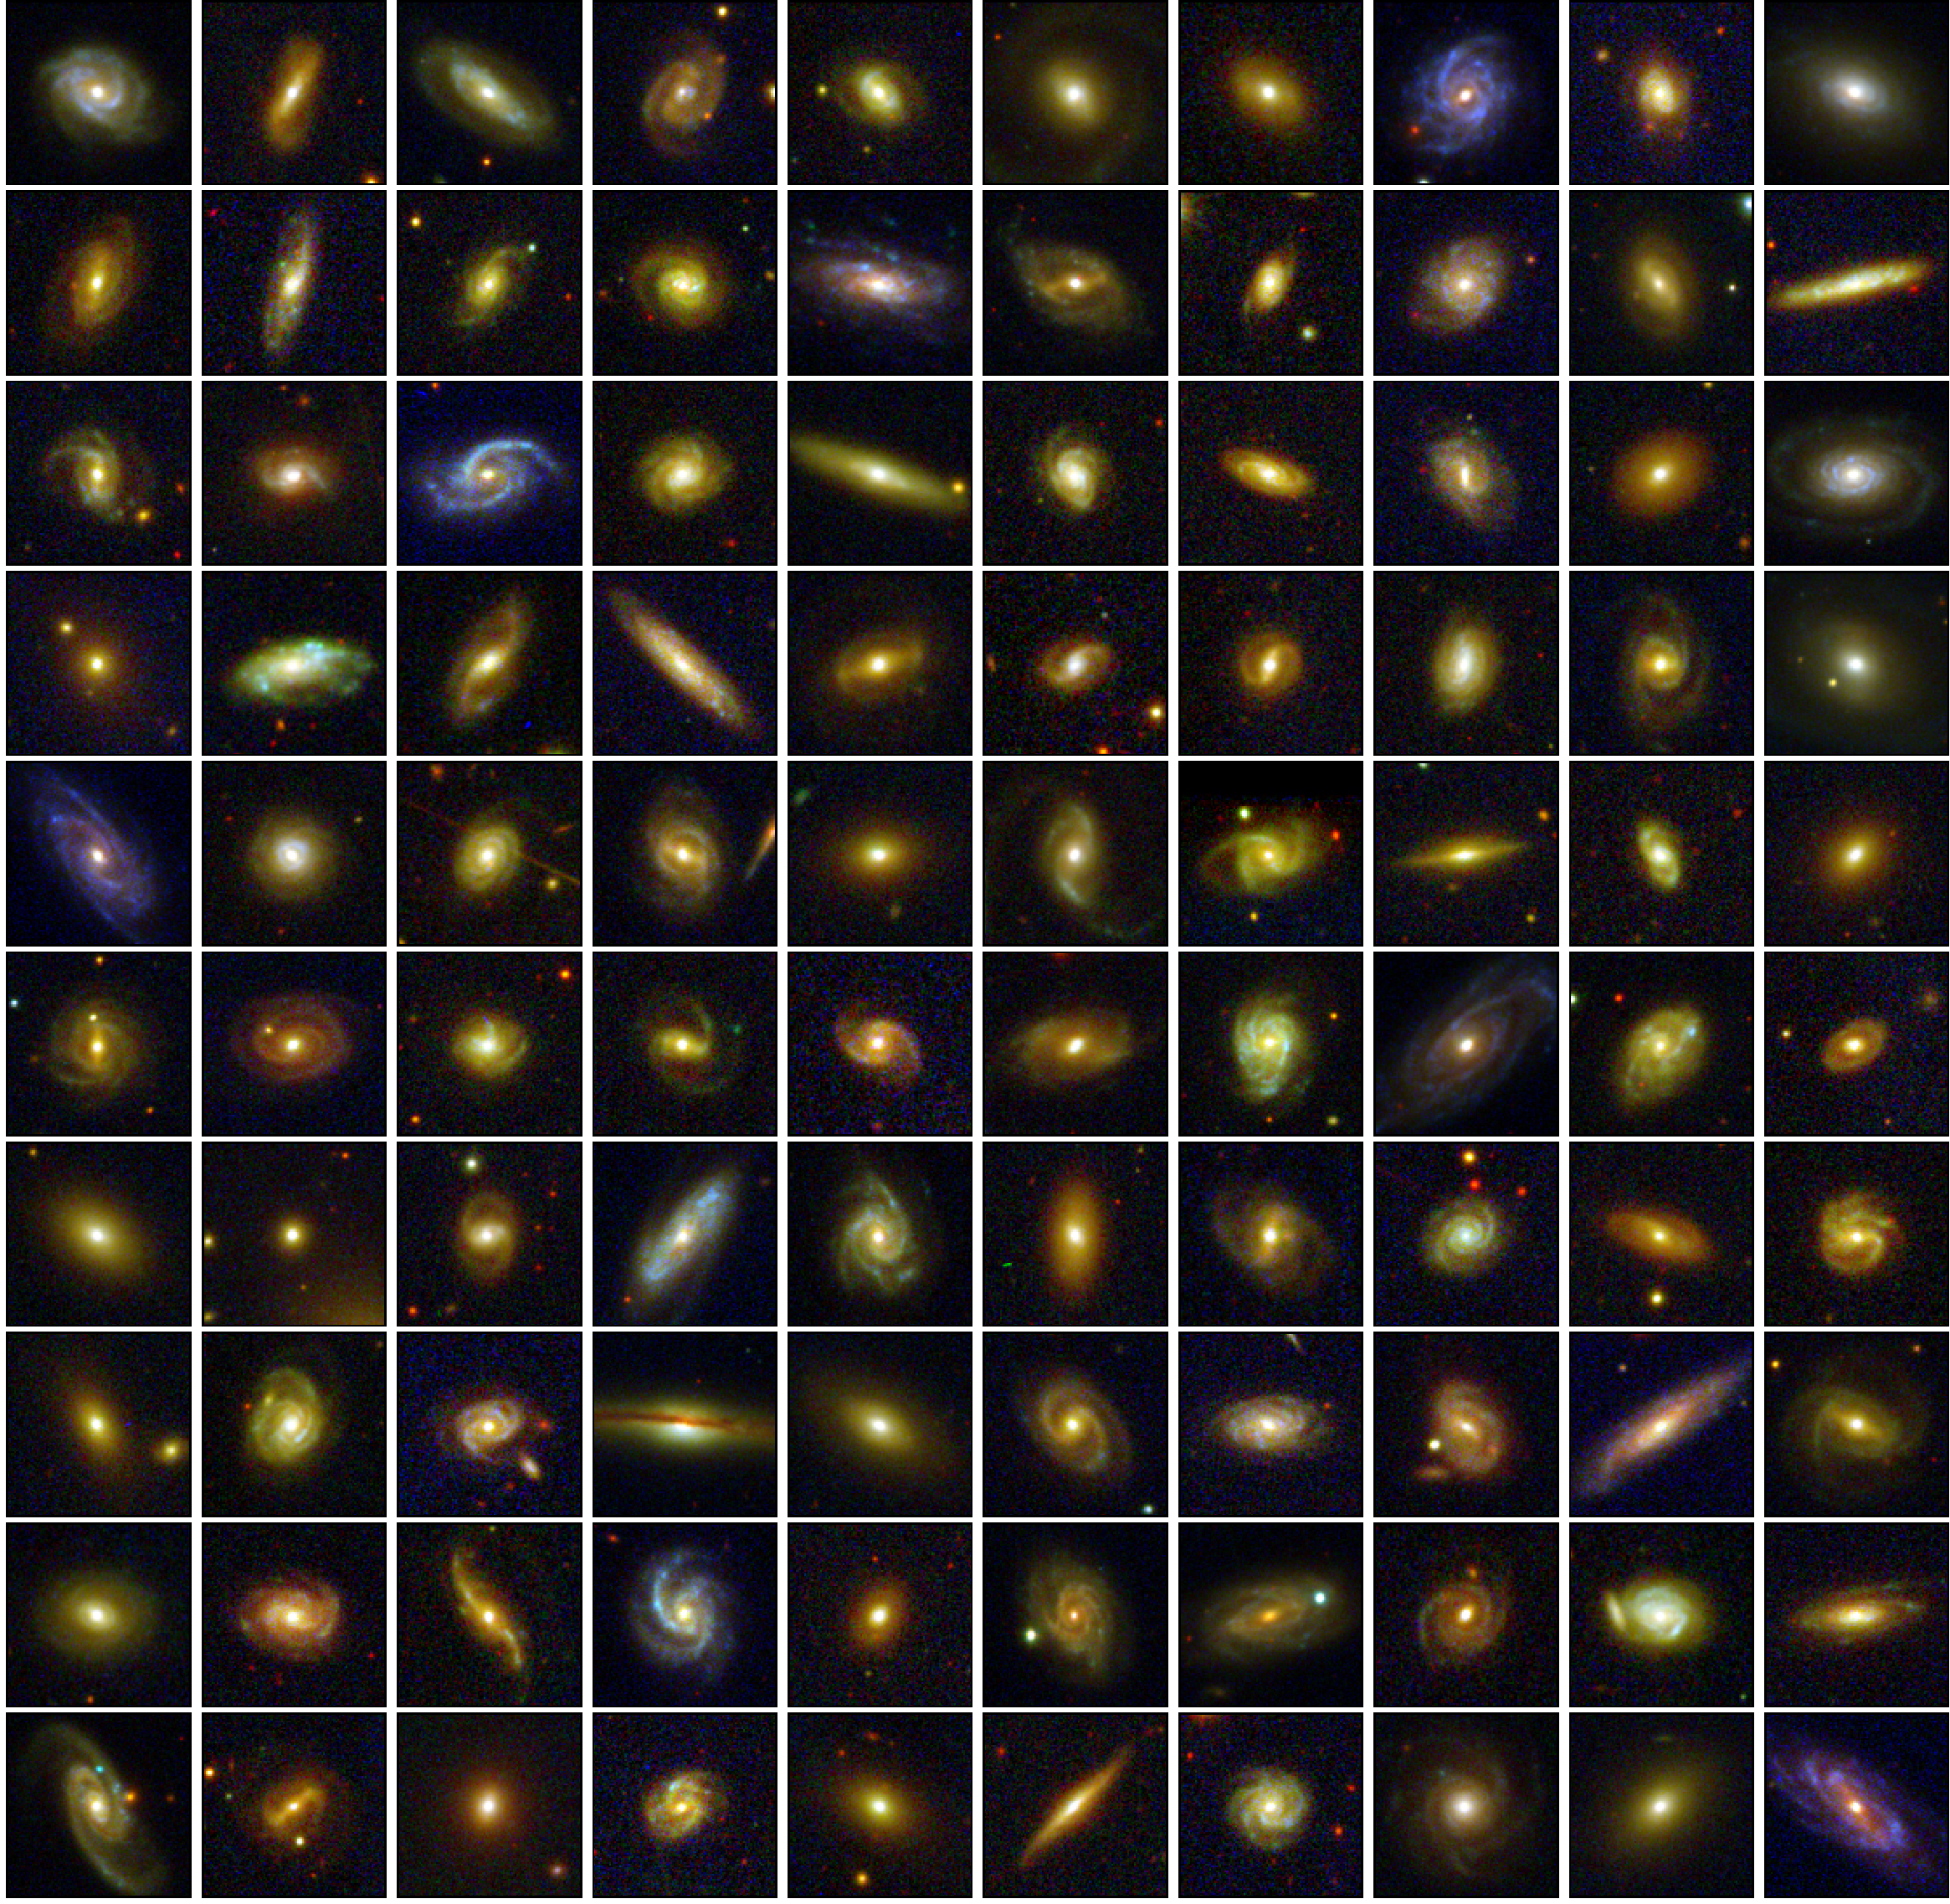
\includegraphics[width=\linewidth,trim={0mm 0mm 117mm 154mm},clip]{figures/galaxygrid_2.pdf}
    \end{figure}
  \end{minipage}\hfill
  \begin{minipage}{0.48\textwidth}
    \begin{center}
      \textbf{Método}
    \end{center}
    \begin{figure}
      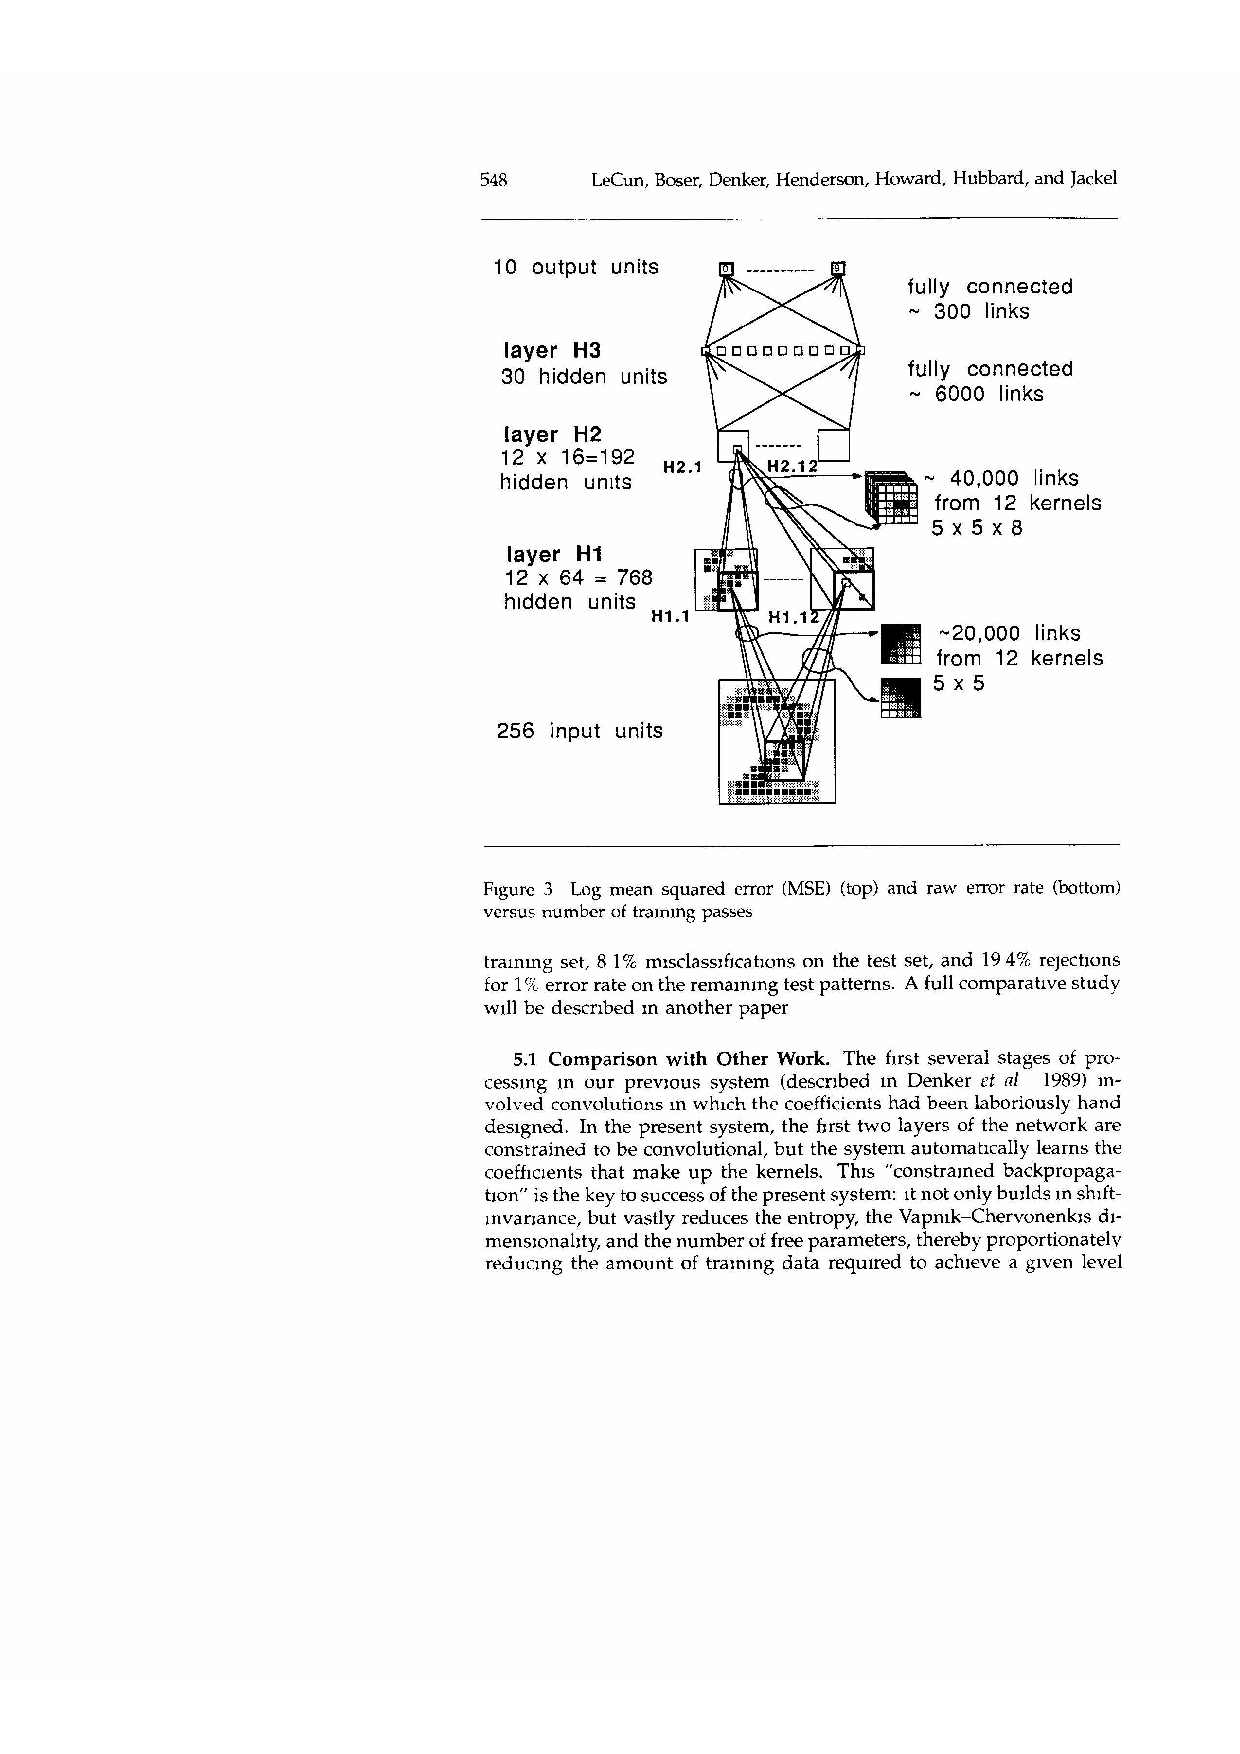
\includegraphics[width=\linewidth,trim={80mm 160mm 18mm 40mm},clip]{papers/lecun-8.pdf}
    \end{figure}
  \end{minipage}
\end{frame}



{
\AtBeginSection{}
\section{Conjunto de Dados}
}

\begin{frame}{S-PLUS: Southern Photometric Local Universe Survey}
  \begin{minipage}{0.48\textwidth}
    \begin{figure}
      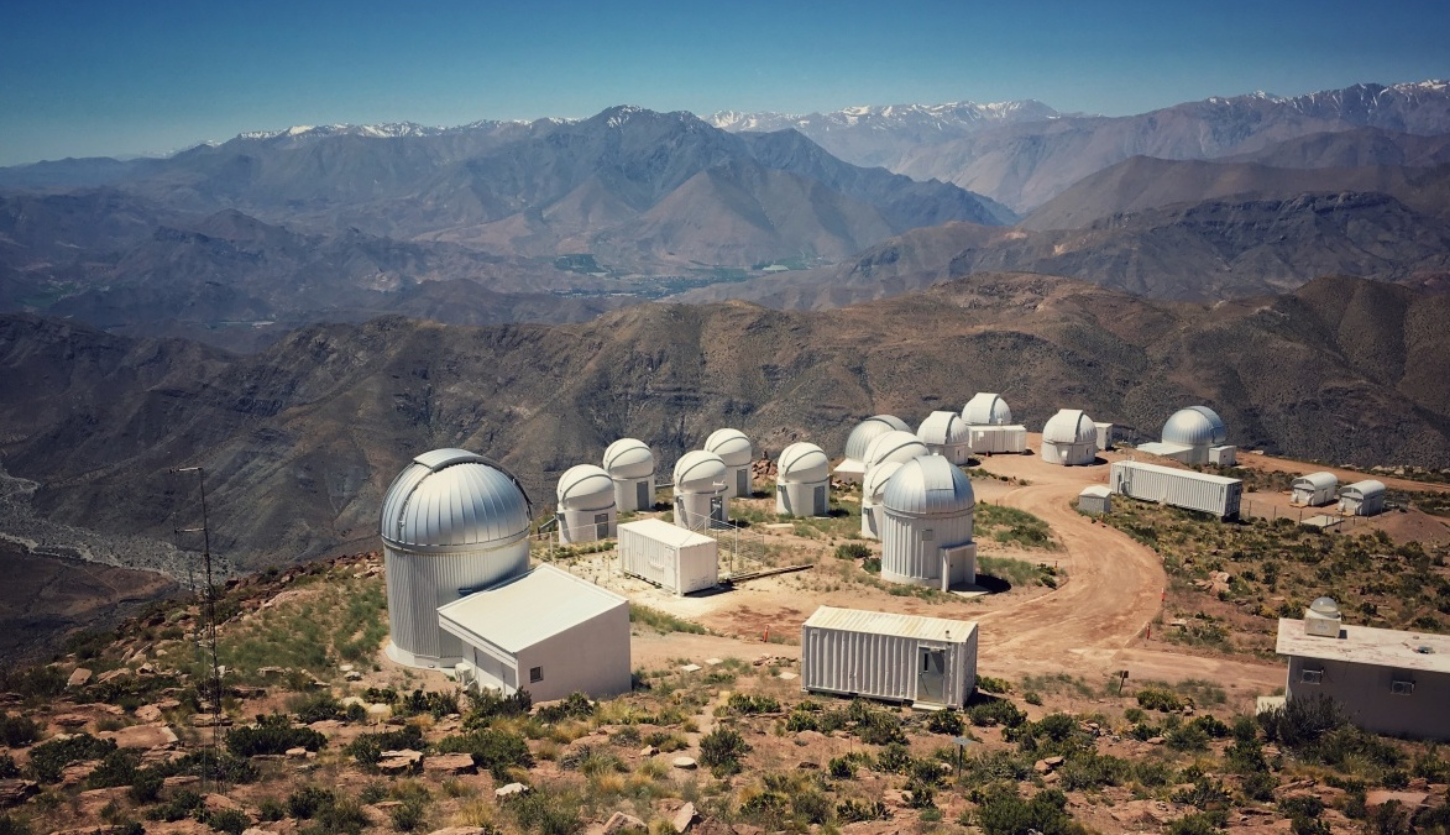
\includegraphics[width=\linewidth,trim={110mm 0mm 40mm 0mm},clip]{fig/splus.png}
    \end{figure}
  \end{minipage}\hfill
  \begin{minipage}{0.48\textwidth}
    \begin{figure}
      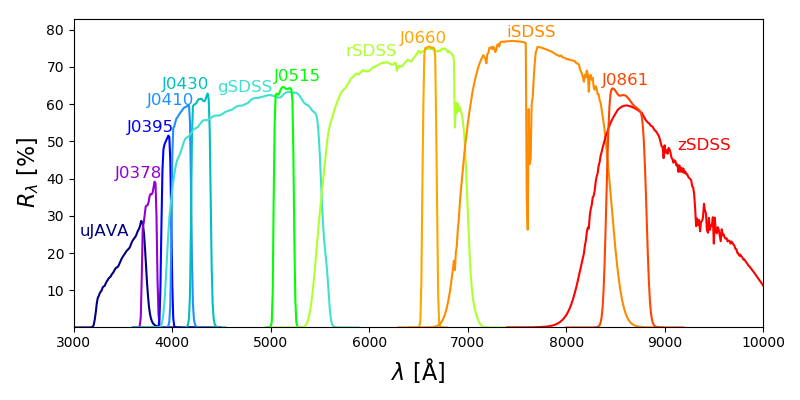
\includegraphics[width=\linewidth]{fig/splus_filters.png}
    \end{figure}
  \end{minipage}
\end{frame}

\begin{frame}{Conjunto de Dados}
  \begin{minipage}{0.53\textwidth}
    \begin{figure}
      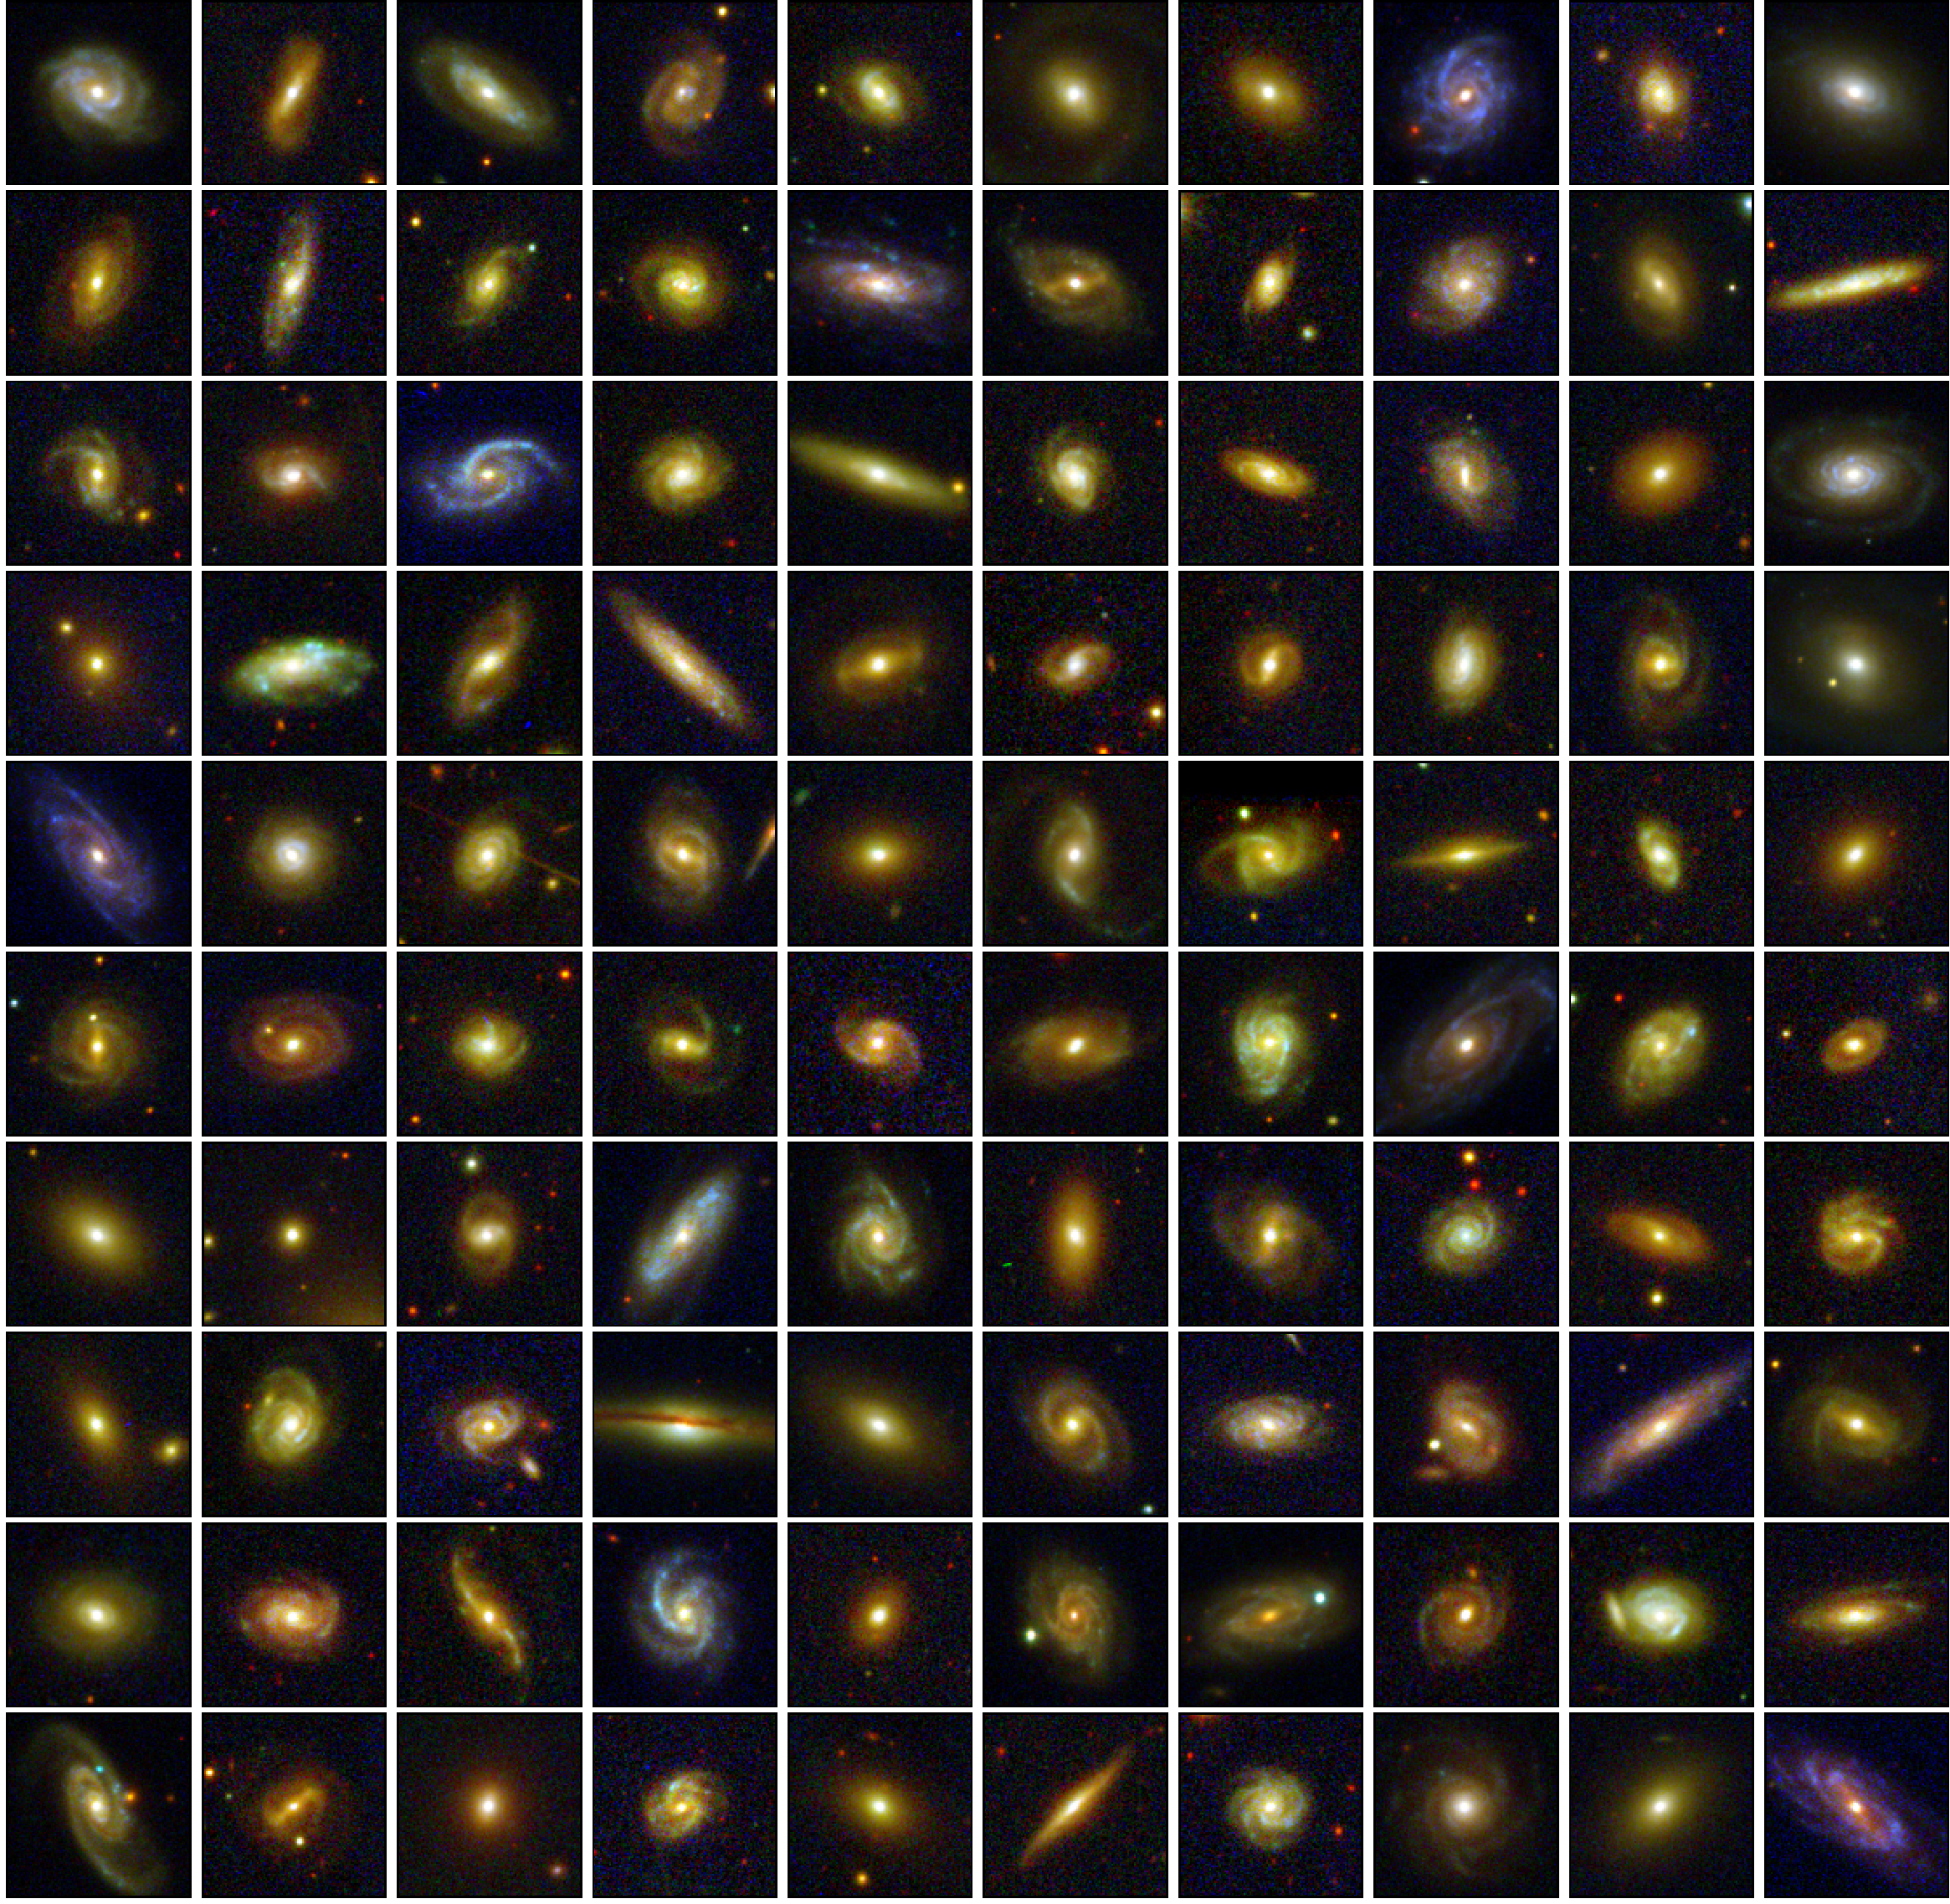
\includegraphics[width=\linewidth]{figures/galaxygrid_2.pdf}
    \end{figure}
  \end{minipage}\hfill
  \begin{minipage}{0.43\textwidth}
    \begin{table}
      \scriptsize
      \begin{tabular}{lrrr}
        \toprule
        Classe   & Treino & Validação & Teste \\
        \midrule
        Elíptica & 714    & 79        & 88    \\
        Espiral  & 1517   & 169       & 188   \\
        Total    & 2231   & 248       & 276   \\
        \bottomrule
      \end{tabular}
    \end{table}
    \begin{figure}
      
\includegraphics[width=0.5\linewidth]{fig/zoo.jpeg}
    \end{figure}
  \end{minipage}

  \vspace{3mm}
  Imagens do S-PLUS e Classificações do GalaxyZoo
\end{frame}

\begin{frame}{Pré-processamento: Redução}
  \vspace{2mm}
  \begin{minipage}{0.48\textwidth}
    \begin{figure}
      \begin{tabular}{ccc}
        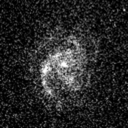
\includegraphics[width=13mm]{imgs/F378.png} &
        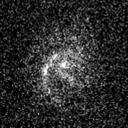
\includegraphics[width=13mm]{imgs/F395.png} &
        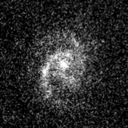
\includegraphics[width=13mm]{imgs/F410.png}   \\
        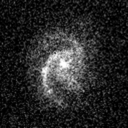
\includegraphics[width=13mm]{imgs/F430.png} &
        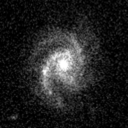
\includegraphics[width=13mm]{imgs/F515.png} &
        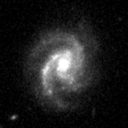
\includegraphics[width=13mm]{imgs/F660.png}   \\
        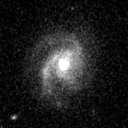
\includegraphics[width=13mm]{imgs/F861.png} &
        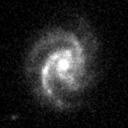
\includegraphics[width=13mm]{imgs/G.png}    &
        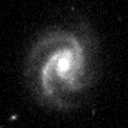
\includegraphics[width=13mm]{imgs/I.png}      \\
        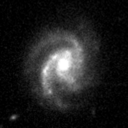
\includegraphics[width=13mm]{imgs/R.png}    &
        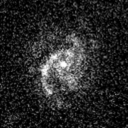
\includegraphics[width=13mm]{imgs/U.png}    &
        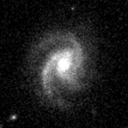
\includegraphics[width=13mm]{imgs/Z.png}
      \end{tabular}
    \end{figure}
  \end{minipage}\hfill
  \begin{minipage}{0.38\textwidth}
    \begin{figure}
      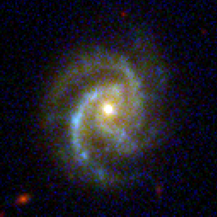
\includegraphics[width=\linewidth]{imgs/color.png}
    \end{figure}
  \end{minipage}
  \captionof{figure}{Imagem em cada banda do S-PLUS e respectiva redução para RGB usando Trilogy.}
\end{frame}

